\begin{figure} [t]
    \vspace{-6pt}
    \centering
    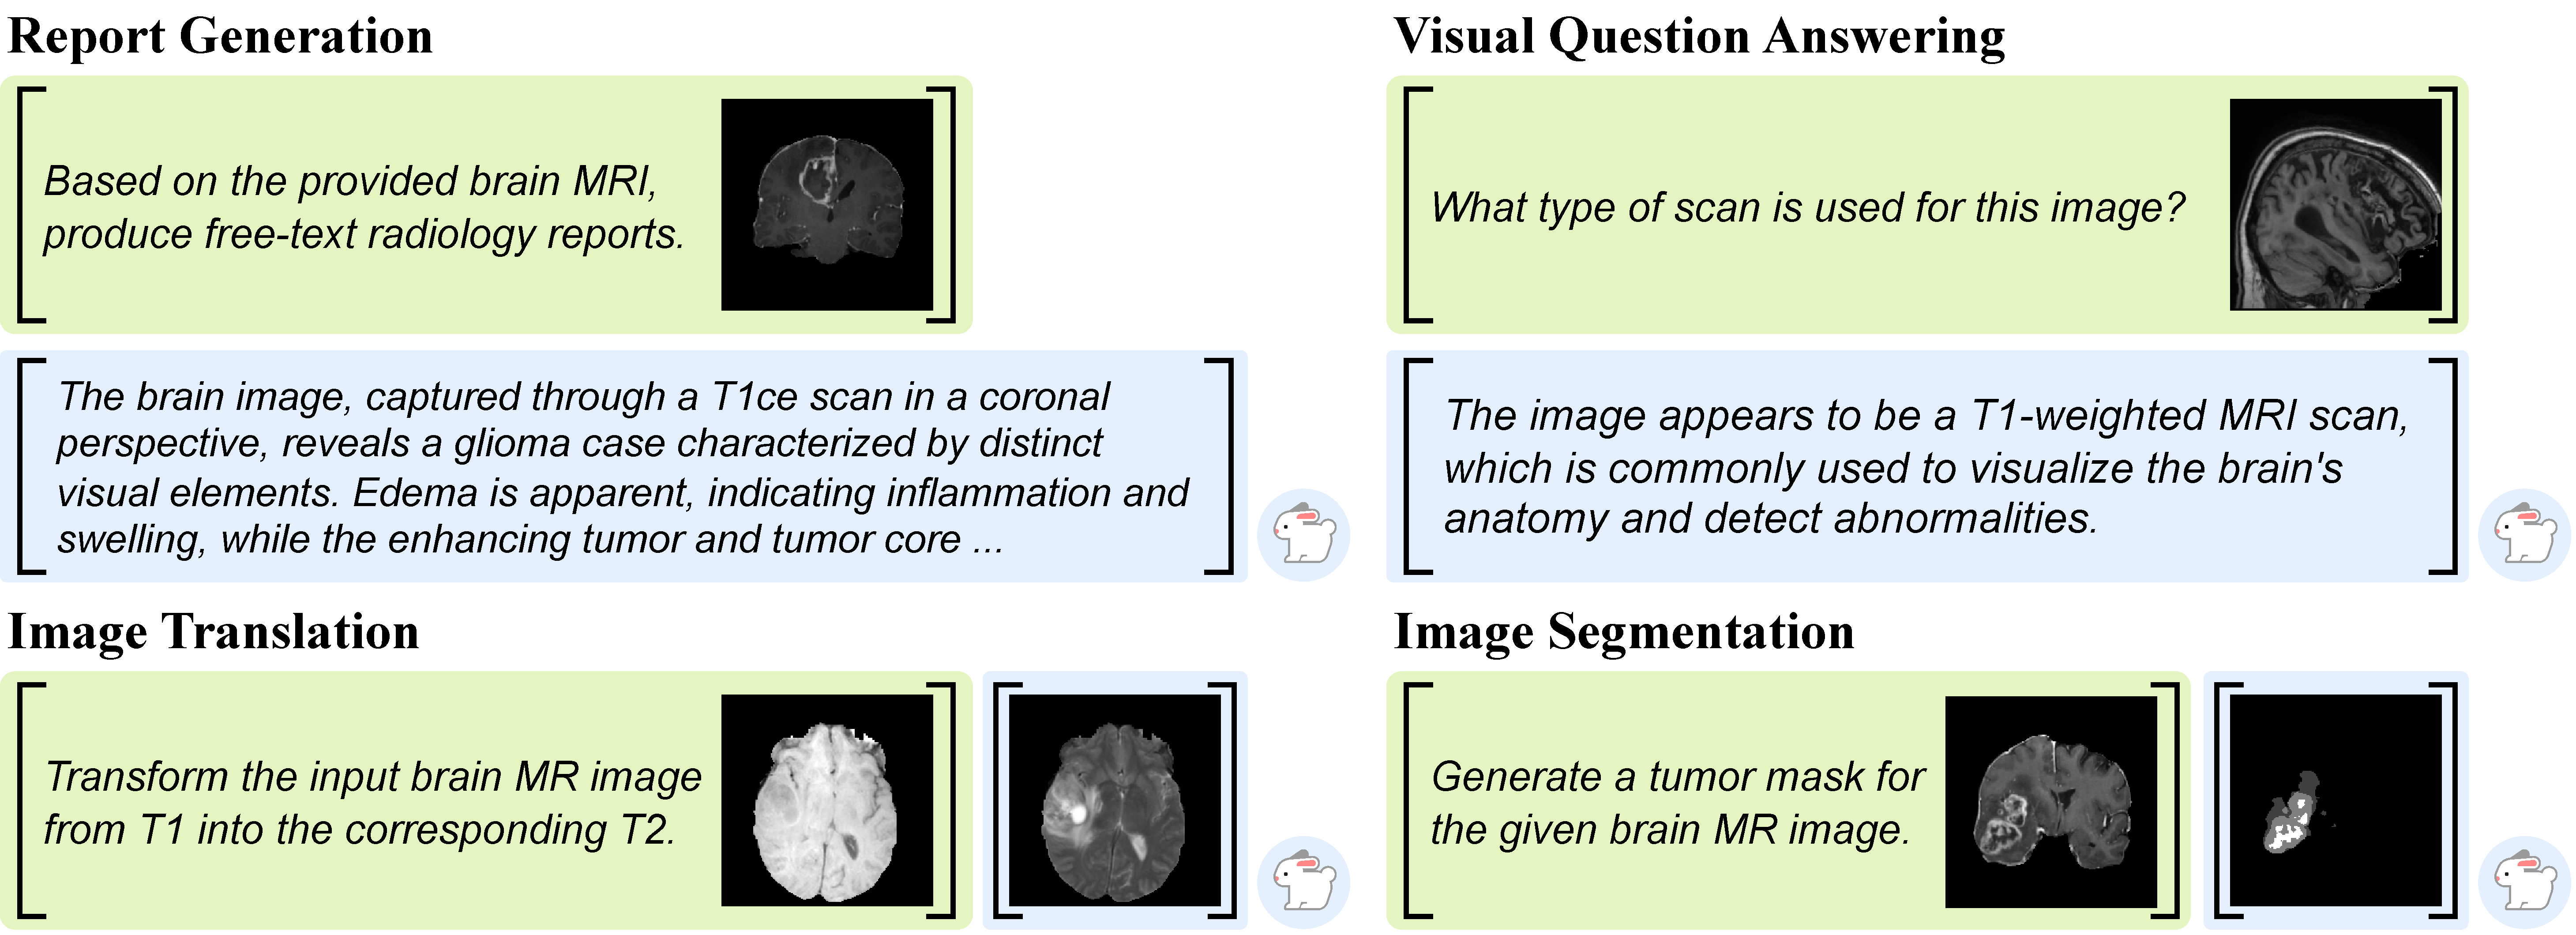
\includegraphics[width=0.99\columnwidth]{figs/fig1.pdf}
    \centering
    \vspace{-3pt}
    \caption{\textbf{Example of LLaBIT performing versatile tasks on brain MR images}. LLaBIT supports report generation and image-to-image tasks.}
    \label{fig1}
    \vspace{-6pt}
\end{figure}

\section{Introduction}
\label{sec:intro}

In recent years, large language models (LLMs) have made significant progress \cite{brown2020language,achiam2023gpt}. LLMs have powerful abilities to understand and reason with natural language, allowing them to adapt to different tasks without being specifically trained for each one. As a next step, there have been attempts to incorporate visual information into language models, enabling them to interpret images with language and to ask and answer questions about visual content \cite{achiam2023gpt,liu2023visual,alayrac2022flamingo}. Methods are being developed for language models to not only process visual information as input, but also to produce it as output \cite{koh2023generating}. These methods have great potential in the medical field, where image understanding requires context, reasoning, and the ability to communicate findings in both text and image. A key method for adapting LLMs to new tasks without losing their original abilities is instruction tuning \cite{brown2020language,wei2022finetuned}. This has proven effective for teaching a model to handle diverse instructions and flexibly apply its knowledge. This idea has been extended to visual instruction tuning \cite{liu2023visual}, enabling LLMs to perform conversational discussions about image content. 
Thus, multimodal LLMs that handle both images and language have emerged \cite{liu2023visual,zhu2024minigpt,chaves2024towards}. The main challenge for these models is to align image features with their powerful, pretrained language-derived features without catastrophic forgetting \cite{koh2023generating,zhu2024minigpt}. This task is even harder with medical images than with natural images, because medical images often appear similar. The model must be able to detect subtle but critical differences in order to provide an accurate description. Furthermore, the region of interest, such as a lesion, is often a small, complex part of the whole image, which makes the task even more difficult. Recent work has explored using VQ-GAN \cite{esser2021taming} to transform medical images like chest X-rays (CXRs) into tokens, integrating them into an LLM without changing its structure \cite{lee2024llmcxr}. This allowed the model to generate both text descriptions and their corresponding images. However, simply generating an image that corresponds to a textual description may have limited clinical use and compressing an image into tokens can lead to a loss of visual details.

In brain magnetic resonance imaging (MRI), diagnosing lesions requires precise decisions from multiple perspectives, often achieved by using different imaging modalities or sequences. These sequences are differentiated by physical acquisition parameters like repetition time and echo time. For instance, T1-weighted images excel at delineating normal anatomy, while T2-weighted images are more sensitive for detecting lesions, as abnormalities like water, edema, and tumors appear hyper-intense \cite{damadian1971tumor,bradley1984comparison}. Leveraging information from two or more sequences enables more precise clinical decisions \cite{cha2006update,ellingson2015consensus}. However, in clinical practice, key sequences may be unavailable due to acquisition time constraints or poor image quality. This necessitates medical image translation (MIT), the task of generating a missing sequence from available ones \cite{kim2024adaptive}. MIT is more clinically relevant than generating images from scratch, aided by LLM guidance \cite{lee2024llmcxr}. Furthermore, identifying the precise location and extent of a lesion through segmentation is critical for accurate diagnosis \cite{kwon2024leveraging,kim2025weakly,kim2025enhancing,kwon2025blood}. Segmentation is also imaging task that can benefit from LLM to segment a region based on a textual description. 

To this end, we propose a method that leverages instruction fine-tuning to align medical images and text, enabling an LLM to perform language-driven visual analysis without compromising its inherent linguistic abilities. Our primary motivation is to create an integrated model that goes beyond simple report generation. We aim to empower a language model to describe images or lesions from the perspective of different MR sequences. Our approach provides a single pretrained language model with four key capabilities: report generation, visual question answering, image translation, and image segmentation for brain MRI. To mitigate information loss from image compression, we propose reusing the encoder features from the VQ-GAN for the two image-to-image tasks. We hypothesize that reusing these feature maps preserves critical image details and thereby improves performance on image-to-image tasks. Our results show that our unified model outperforms specialized models designed for each task, demonstrating the significant potential of a text-and-image integrated language model. Representative samples of our model, Large Language Model for Brain Image Translation (\textbf{LLaBIT}), are shown in Figure \ref{fig1}.

\noindent \textbf{Our contributions}
\begin{itemize}[noitemsep, topsep=0pt, partopsep=0pt, parsep=0pt]
    \item[1.] We integrate images into our language model to give it the ability to translate and segment images without losing its language reasoning ability. 
    \item[2.] We reuse the feature map of the encoder along with a zero-skip connection to improve the quality of image-to-image tasks.
    \item[3.] We evaluated our model on text generation, visual question answering, image translation, and image segmentation across five datasets that include brain lesions such as tumors. Our model achieved superior performance in all tasks, showing that a language model can be effectively utilized for not only image-to-text but also image-to-image tasks.
\end{itemize}